\documentclass[10pt]{article}
\usepackage{makeidx}
\usepackage{multirow}
\usepackage{multicol}
\usepackage[dvipsnames,svgnames,table]{xcolor}
\usepackage{graphicx}
\usepackage{epstopdf}
\usepackage{ulem}
\usepackage{hyperref}
\usepackage{amsmath}
\usepackage{amssymb}
\author{Felipe Vásquez Moraga}
\title{PROPOSAL ABSTRACT POSTDOCTORADO 2018}
\usepackage[paperwidth=612pt,paperheight=792pt,top=28pt,right=34pt,bottom=35pt,left=34pt]{geometry}


\begin{document}

\noindent \textbf{PROPOSAL ABSTRACT:}

\noindent \textbf{}

{\raggedright
\vspace{3pt} \noindent
\begin{tabular}{|p{514pt}|}
\hline
\parbox{514pt} {\raggedright\vspace{3pt}
The maximum length of this file is \textbf{10 pages} (Must use letter size, Verdana size 10 or similar)\textbf{. }For an adequate evaluation of your proposal merits,this file must include the following aspects: Proposal description, Bibliographical References, Hypothesis, Goals, Methodology, Work Plan, Work in progress (if applicable) and Available Resources.
Make sure to describe the relevance of the proposal topic in relation to the state of the art in the field.
Keep in mind the Bases del Concurso FONDECYT de Postdoctorado 2018 and Application Instructions.} \\
\hline
\end{tabular}
\vspace{2pt}

}

%\section{Proposal}
\section{Introduction}
%\section{Introducción}
%Como consecuencia del crecimiento explosivo de la WEB, la integración de motores de búsqueda como Google en computadoras personales y dispositivos móviles, y del uso de la redes sociales, la tarea de agrupamiento automático de texto, e.g. Tweets o documentos en un motor de búsqueda, resulta cada vez de mayor importancia debido a la necesidad de revelar las categorías subyacentes en grandes volúmenes de datos. La generación de grandes cantidades de documentos sobrepasa hoy en día las capacidades de computadores personales e incluso de equipos de cómputo de alto desempeño. 
As a consequence of the explosive growth of the WEB, the integration of search engines such as Google into personal computers and mobile devices, and the wide use of social networks, the task of clustering text data, i.e. Tweets or documents in a search engine, has each time an increasing importance because of the necessity of unraveling the underlying categories in large volumes of text data. Nowadays the generation of large amounts of documents surpasses the computational power of personal computers and even of high performance computers.
%A modo de ejemplo, se estima que la cantidad de páginas WEB que motores de búsqueda populares como Google o Yahoo indexan es del orden de las decenas de billón.
As an example, it is estimated that the amount of WEB pages that popular search engines such as Yahoo! and Google index is higher than the tens of a billion.
%Es por lo tanto de gran interés poder desarrollar técnicas capaces de automáticamente organizar, clasificar y resumir colecciones de documentos que se encuentren distribuidas en múltiples máquinas de una red, y que a su vez hagan uso eficiente del hardware moderno, en particular del paralelismo existente en las arquitectura multi-núcleo (multi-core). En problemas reales como  \textit{Collection Selection} para colecciones distribuídas, en donde para una consulta dada se debe identificar la colección más adecuada dentro de la cual se buscaran documentos relevantes \cite{CM13}, los desafíos relacionados con la escalabilidad y eficiencia en los métodos de \textit{Knowledge Discovery} se han vuelto de gran importancia. Los algoritmos tradicionales operan usualmente con conjuntos de datos cargados completamente en memoria principal. De ahí que puedan realizar operaciones de cálculo de distancias entre pares de documentos de manera muy rápida, visitando cada dato muchas veces. Cuando el tamaño de la colección es mucho mayor a la cantidad de memoria RAM disponible, ya sea por la cantidad de documentos o también por el tamaño de cada uno, este proceso es impracticable debido a restricciones de espacio o capacidad de cómputo.
It is therefore of great interest to develop algorithmic techniques capable of automatically organize, classify and summarize document collections distributed in multiple machines of a network, and that also perform efficiently in modern hardware, particularly within parallel processing frameworks in multi-core architectures. In real problems such as \textit{Collection Selection} for distributed document databases, in which for a given query the computer node containing the most suitable
sub-collection must be selected to answer it~\cite{CM13}, the challenges related to the scalability and efficiency of \textit{Knowledge Discovery} methods have become very important. Traditional algorithms often assume that the whole dataset is loaded into main memory (RAM) and thus every document can be accessed at any time with no access latency. In scenarios where the size of the collection is much bigger than the amount of available RAM either because of the number of documents or the length of each document, this ideal loading process is unfeasible due to real constraints in the storage or computational capabilities.

%A menudo, el texto se estructura en colecciones digitales de documentos cuya extensión (cantidad de caracteres) es variable, e.g. las páginas WEB o el contenido generado por los usuarios de redes sociales como Twitter. Para permitir el procesamiento de estas colecciones, primero se extrae el conjunto de palabras que aparece en ella y se ordena lexicográficamente; a este conjunto ordenado se le denomina vocabulario. Luego, el contenido de cada documento es representado algebraicamente por un vector, donde cada componente corresponderá a una de las palabras del vocabulario y cuyos valores estarán dados por las frecuencias de ocurrencia de cada palabra respectiva en el documento. Como consecuencia de la riqueza léxica del lenguaje, la cardinalidad del vocabulario es en general muy grande en comparación con los tamaños usados habitualmente por los algoritmos tradicionales de reconocimiento de patrones, i.e. partiendo del orden de los miles hasta los millones de palabras. Debido a esto, la tarea de agrupamiento automático de documentos tiene un alto costo de cómputo (tiempo de uso del procesador) y de almacenamiento (cantidad de memoria RAM y disco usado). Si a lo anterior se agrega que las cantidades de documentos en una colección puede superar los millones, entonces tanto las técnicas tradicionales de procesamiento, agrupamiento,  así como también las capacidades computacionales actuales  de una sola máquina resultan insuficientes o en el mejor de los casos los tiempos de respuesta son excesivos.
Often, text data is structured in digital collections of documents whose length (number of characters) is variable, e.g. WEB pages or the content generated by users in social networks such as Twitter or Facebook. In order to enable the processing of these collections, in a first stage of preprocessing a set of words occurring in the documents are extracted and sorted in lexicographical order; this word set is referred to as the Vocabulary. Then, the content of every document in the collection is represented as a vector in which each dimension denotes a specific word of the Vocabulary and its value in a document vector is given by a function of the number of occurrences of the word within the document and the number of documents in which it appears. As a natural consequence of the lexical richness of every language, the size of the Vocabulary, and in turn the dimensionality of the vector space onto which a document is represented,  is far bigger than the data size that traditional clustering algorithms manage. Because of this, the task of automatic document clustering has high computational and storage (RAM and secondary memory) costs. Along with this, when the number of documents is large (tens or hundreds of thousand and even millions of items) then traditional techniques for processing and clustering documents, and current computational capabilities of a single machine and also high performance machines are insufficient. Even in the most favorable scenario the storage and computational power tackle the challenge but the response time are excessive.

%Existe tres enfoques exitosos para la construcción de algoritmos de agrupamiento sobre grandes volúmenes de datos. El primero consiste en introducir restricciones en la cantidad de accesos a un documento (una sola pasada), el segundo en usar el paralelismo disponible en las arquitecturas multi-core actuales o usar GPUs (tarjetas gráficas) y por último, particionar el conjunto de datos en mútlples máquinas para su procesamiento distribuido.
There exist three approaches successfully applied to the construction of clustering algorithms capable of processing large volumes of data. The first one introduces constraints on the number of passes allowed on a document (related to the amount of time it is loaded into main memory). The second one exploits current multi-core architectures to perform parallel processing of the data, which does not solve the massive volume problem. The last one combines the computational power of a single machine together with the scalable storage capability of a distributed system by partitioning the dataset into several independent machines connected through a network.

%Esta última línea de trabajo es promisoria dado que permite aprovechar las capacidades locales de computadores que no necesariamente deben ser servidores de gran escala con múltiples procesadores. Dentro de este enfoque existen dos contextos respecto del origen de los datos que deben ser diferenciados. Por una parte, existen problemas donde la estrategia usada para hacer frente al gran volúmen de datos consiste en distribuirlo entre distintos computadores, lo que conlleva un traslado de datos durante la ejecución del algoritmo \cite{N15}. Por otra parte, existe otro contexto en el que los datos se encuentran naturalmente distribuídos, e.g. colecciones documentales locales a distintas zonas geográficas, y donde además no es posible  centralizarlos, debido a costos de transmisión o por motivos de privacidad \cite{JW05,LHLX12}.
The last above mentioned approach seems promising since it allows to exploit the local capabilities of single computers with multi-core architectures without sacrificing scalability to large data volumes because of its distributed design. Within this path there are two contexts regarding the data generation scenario. On the one hand, in some problems where the dataset is large but collected in a centralized fashion, the strategy employed consists in partitioning the collection into several
machines or nodes of a network. This scheme leads to the transmission of a lot of data during the execution of the algorithm~\cite{N15}. On the other hand, there are some problems where the data is generated in a distributed fashion and where besides it is not feasible to centralize the data because of high transmission costs or privacy issues~\cite{JW05,LHLX12}, e.g.\  search engines  work with document collections originated and stored in different geographical locations.



\section{Problem Definition and State of the Art}
%\section{Definición del Problema y Estado del Arte}
%Sea $X=\{X_1,X_2,\ldots ,X_p\}$ una colección de documentos donde \(\bigcup_{i=1}^p X_i=X\) y \(\forall i\neq j \in [1,\ldots ,p], X_i\cap X_j=\emptyset\). Esta colecci\'on se encuentra dividida en $p$ máquinas distinas, y a su vez, cada subconjunto $X_i$ se encuentra compuesto por $n_i$ vectores en $\mathbb{R}^d$. 
Let $X=\{X_1,X_2,\ldots ,X_p\}$ be a collection of documents where\(\bigcup_{i=1}^p X_i=X\) and \(\forall i\neq j \in [1,\ldots ,p], X_i\cap X_j=\emptyset\). This collection is partitioned into $p$ different machines of a network, and also each subset $X_i$ consists of $n_i$ vectors in $\mathbb{R}^d$. Additionally, in a distributed environment, data sites may be homogeneous or heterogeneous, depending if different sites contain data for exactly the same set of features or for different set of features respectively.  
%La tarea de Clustering distribuído consiste en obtener un conjunto de $k$ particiones \(C_1,C_2\ldots,C_k\) donde \(\bigcup_{i=1}^k C_i=X\) y además \(\forall i\neq j \in [1,\ldots ,k], C_i\cap C_j=\emptyset\), tal que cada una de ellas represente una o una parte de una categoría temática de la colección completa y a su vez todas las categorías esten representadas en los grupos o clusters $C_i$. Expresado de una manera distinta, esto significa que cada cluster contiene documentos más similares entre sí según su contenido que los que están en otros clusters.
The distributed data clustering task consists in obtaining $k$ data partitions \(C_1,C_2\ldots,C_k\) where \(\bigcup_{i=1}^k C_i=X\) and also \(\forall i\neq j \in [1,\ldots ,k], C_i\cap C_j=\emptyset\), such that each one of them represents a topical category of the overall collection and in turn all the categories are covered by the partitions or clusters $C_i$. Expressed in a different manner, this means that every cluster contains more similar documents according to their content in comparison to the other ones contained in different clusters.
%La similaridad entre vectores respresentates de documentos es usualmente medida mediante una función $S:\mathbb{R}^d\times \mathbb{R}^d\rightarrow[0,1]$ como por ejemplo la denominada similaridad del coseno:\[S(x_a,y_b)=\frac{<x_a,x_b>}{\|x_a||x_b|}\], donde $<u,v>$ con $u,v\in\mathbb{R}^d$ denota el producto interno entre dos vectores y $|u|$ es la norma euclideana del vector.
The similarity between document vectors is usually measured by means of a function $S:\mathbb{R}^d\times \mathbb{R}^d\rightarrow[0,1]$, e.g.\  the cosine similarity function: \[S(x_a,y_b)=\frac{<x_a,x_b>}{\|x_a||x_b|},\] where $<u,v>$ with $u,v\in\mathbb{R}^d$ denotes the inner product between two vectors and $|u|$ corresponds to the Euclidean norm of a vector.
%En pocas palabras, esta tarea consiste en encontrar una estructura de grupos compactos respecto a la similaridad entre sus miembros y homogéneos respecto de su contenido, de acuerdo a alguna medida de similitud como puede ser la del coseno.
In a nutshell, this task consists in finding a structure of compact and homogeneous groups with respect to a similarity value between their members that accounts for their content. 

%El modo general de operación de las técnicas de clustering sobre colecciones de datos distribuídas consiste de cuatro etapas: Inicialmente el conjunto de datos se encuentra particionado en varios nodos. Luego cada nodo genera un modelo de agrupamiento sobre su respectivo subconjunto local. Estos modelos son transmitidos a un nodo central (e.g. puede ser un conjunto de representantes identificados en cada grupo), el cual combina los modelos locales en una solución global. Opcionalmente, el modelo global puede ser transmitido a los otros nodos para que estos refinen sus modelos locales y se genere un nuevo modelo global depurado siguiendo las mismas etapas ya mencionadas. Este esquema se representa gráficamente en la figura
An overall operation mode of the distributed data clustering techniques consists of four stages: Initially, the dataset is partitioned into several nodes. Next, each node generates a clustering model over its corresponding local subset. These local models are then transmitted to a central node (e.g.\ A model can consists of representative points identified from a local clustering), which integrates the local models in a global solution. Eventually, this global model can be re-transmitted to the 
other nodes in order to refine their local models and then, by performing the same previous steps, a new depurated 
global model is built. This scheme is depicted in Figure~\ref{fig:distributed_clustering}.

\begin{figure}[!h]
\centering
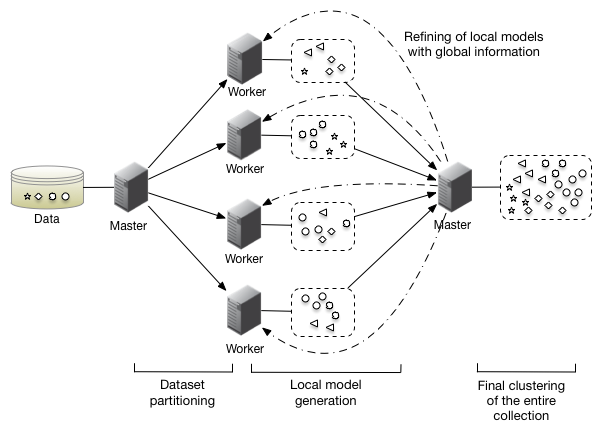
\includegraphics[width=0.9\textwidth]{./figs/distributed_data_clustering_scheme_en.png}
%\caption{Esquema general del funcionamiento de las técnicas de clustering sobre datos distribuídos.}
\caption{Overall scheme of operation of the distributed data clustering techniques.}
\label{fig:distributed_clustering}
\end{figure}

%\subsection{Enfoques paralelos y distribuídos para el agrupamiento de datos masivos y de alta dimensionalidad}
\subsection{Parallel and distributed approaches for massive and high dimensional data clustering}
%Hasta donde sabemos, gran parte de los esfuerzos en la literatura para la construcción de técnicas de agrupamiento capaces de operar en entornos donde los datos están distribuídos se ha enfocado en datos con datos cuya dimensionalidad es relativamente baja (menos 100 atributos) en comparación con las colecciones documentales (más de $10^4$ atributos). Sin embargo, a continuación detallamos los principales avances en el área de agrupamiento sobre datos distribuídos, destacando aquellas contribuciones dirigidas a los datos con alta dimensionalidad en sus representaciones computacionales.
As far as we know from the literature, most of the existing efforts for the construction of clustering techniques capable of operating in scenarios where the data is distributed have been focused on low dimensional data (less than 100 attributes) in contrast with document datasets in which a document vector for a small collection may have about $10^4$ attributes. Nevertheless, the main advances in distributed data clustering are detailed below, specially highlighting those contributions focused on methods capable of dealing with high dimensional data.
\begin{enumerate}
%\item Principales contribuciones en algoritmos paralelos
\item Main contributions on parallel algorithms
%\cite{XJK99} y \cite{DM99} proponen extensiones paralelas para los algoritmos DBSCAN y K-Means respectivamente. Otro enfoque escalable basado en memoria secundaria consiste en diseñar algoritmos capaces de operar dentro del marco de Mapreduce. En este contexto, es posible destacar las contribuciones de \cite{DDGR07} que proponen una implementación del algoritmo EM y también de \cite{EIM11} que consideran el problema de las K-Medianas en Mapreduce\footnote{Hadoop MapReduce es un software que permite escribir aplicaciones que procesen grandes cantidades de datos (terabytes) en paralelo sobre grandes Clusters de computadores.}. Otro enfoque paralelo para K-Means se presenta en \cite{BMVKV12} y se denomina K-Means$++$. También destaca, por los volúmenes de documentos procesados, la técnica EM-Tree propuesta por \cite{VVGN15} (cientos de millones de páginas WEB).
\cite{XJK99} and~\cite{DM99}  propose parallel extensions for the algorithms DBSCAN and K-Means. Another scalable approach based on secondary memory consists in designing algorithms capable of working within the Mapreduce framework\footnote{Hadoop MapReduce is a software solution that enables the construction of applications capable of processing large amounts of data (e.g. Terabytes) in a parallel fashion over big computer clusters.}. In this context it is possible to highlight the contributions made by~\cite{DDGR07} in which they propose an implementation of the EM algorithm and also by~\cite{EIM11} in which they tackle the K-Median problem by using Mapreduce. Another parallel approach for K-Means is presented by~\cite{BMVKV12} and it is called K-Means$++$. Additionally, the EM-Tree proposed by~\cite{VVGN15} is very interesting since it allows to process very large datasets, specifically the authors show that it can handle hundred of millions of WEB pages.

%\item Enfoques que consideran alta dimensionalidad
\item Approaches capable of dealing with high dimensional data
%En \cite{KHSJ01} los autores proponen un método para obtener componentes principales sobre datos heterogéneos distribuídos. Aprovechando este primer avance, también proponen un método de clustering que opera sobre conjuntos de datos heterogéneos y de alta dimensionalidad. Una vez obtenidas las componentes principales globales, se proyectan los datos locales de cada nodo y se aplica una técnica tradicional de clustering sobre estos. Finalmente, un nodo centraliza los clusters identificados y los combina para obtener el agrupamiento global. 
\cite{KHSJ01} propose a method to obtain the Principal Components (PCA) over heterogeneous and distributed data. Based on this contribution on dimensionality reduction they also propose a clustering method that works over high dimensional data. Once the global principal components are obtained by using the distributed method and transmitted to each node, local data are projected onto the components and then a traditional clustering technique is applied. Finally, a central node integrates the local clusters in order to obtain a global clustering model.
%Varios años más tarde, \cite{LBK13} presentan otro algoritmo de computo de componentes principales (PCA) sobre datos distribuídos. Para esto, cada nodo calcula PCA sobre sus datos locales y envía una fracción de estos, los que serán usados por un nodo central para estimar los componentes principales globales. Estos componentes globales son re-enviados a cada nodo. Luego, los datos locales de cada nodo serán proyectados, y estas proyecciones serán usadas para calcular un coreset mediante un algoritmo distribuído. Este coreset global construído sobre los datos proyectados será usado para la obtener la solución del clustering global.
Several years later,~\cite{LBK13} present another algorithm for principal components extraction over distributed data. To this end, each node computes PCA over its local data and transmit a fraction of them to a central node. This node uses the received components to estimate the global principal components, which are later transmitted to each node. After this, in every node, local data are projected onto the global components and the projected data are used for computing a coreset by means of a distributed algorithm. The global coreset built from the local projected data will be finally used to obtain a global clustering model.  

%\cite{LZO03} proponen un algoritmo denominado D-CoFD para datos de alta dimensionalidad distribuídos tanto homogéneos como heterogéneos.
\cite{LZO03} propose an algorithm called D-CoFD for high dimensional and distributed data that also is capable of dealing with homogeneous and heterogeneous environments.

%\item Enfoques basados en densidad
\item Density based approaches
%\cite{JKP03} proponen una técnica de clustering por densidad para datos distribuídos homogéneos. Los nodos construyen modelos locales y transmiten un conjunto de representates de cada cluster encontrado a un nodo central. En el nodo central se realiza un nuevo clustering sobre los representates, modelo que es retransmitido a los nodos locales para su actualización.
\cite{JKP03} propose a distributed data clustering technique in which local nodes build models and transmit a set of representatives of each cluster to a central node. In this node a centralized clustering method is applied over the representatives and then the resulting model is re-transmitted to the local nodes to update their models.
%\cite{KLM03} proponen una técnica de clustering sobre conjuntos de datos distribuidos homogeneos basada en estimadores de densidad.
\cite{KLM03} propose a clustering technique based on density estimates.
%\cite{JKP04} proponen una versión de DBSCAN escalable y capaz de operar sobre colecciones distribuidas. Primero se seleccionan los mejores representantes locales dependiendo de que tantos datos representan en cada nodo y se envian a un nodo central. Este nodo agrupa estos representantes y los envía a cada nodo para que estos asocien sus datos locales a aquellos representantes más cercanos.
\cite{JKP04} present a scalable version of DBSCAN that is also capable of operating over distributed collections. First, the best local representatives a selected depending on the number of points that each one represents and then those chosen points are sent to a central node. This central node clusters the received local representatives into a single new model, which is re-transmitted to the other nodes so they can improve their local group structure.

%\item Enfoques basados en modelos paramétricos
\item Approaches based on parametric models
%\cite{MG03} Proponen un método de clustering sobre datos distribuídos que combina múltiples modelos paramétricos generados por varios nodos sobre subconjuntos de datos. El foco de este trabajo recae también sobre el cuidado de la privacidad de los datos.
\cite{MG03} propose a clustering method that combines local parametric models, each one built on a single node, into a general one. The main contribution of this work consists in a method capable of dealing with distributed data that also considers the privacy of the local data in each node, since it transmits a summary of each local data and not raw points.
%\cite{KKPS05} proponen una técnica de clustering sobre datos distribuidos basada en un modelo paramétrico. Localmente, se identifican modelos de mezcla de gaussianas usando el algoritmo EM. Posteriormente, se mezclan estos modelos gaussianos locales para generar un modelo global.
\cite{KKPS05} present a technique that fits a Gaussian mixture model in each node using the EM algorithm. Finally, all these Gaussian mixture models are integrated into a general parametric model.

%\item Enfoques basados en representantes
\item Approaches based on representative points
%\cite{FZ00} extienden esquemas paralelos basados en centroides para soportar la identificación de grupos sobre datos distribuídos. Específicamente extienden K-Means, K-Harmonic-Means y EM.
\cite{FZ00} extend centroid based techniques to identify groups over distributed data. Specifically, they extend K-Means, K-Harmonic-Means and EM.
%\cite{ZLW08} proponen una técnica para la construcción de K-Medianas aproximadas sobre datos distribuidos en el escenario de streaming en que los datos se reciben de manera continua.
\cite{ZLW08} propose an approximate K-Median clustering technique that works over stresaming data, i.e.\ data is continuously collected. 
%\cite{BEL13} presentan técnicas de clustering basadas en centroides para datos distribuídos. Para esto proponen un método de construcción de coresets sobre datos distribuidos para K-Medias y K-Medianas.
\cite{BEL13} address the distributed clustering problem by using centroid based techniques that use a novel coreset construction method that works for distributed data.
%\cite{NC14} utilizan algoritmos evolutivos para solucionar dos problemas de K-Medias sobre datos distribuidos: La selección de prototipos iniciales y la identificación de la cantidad de clusters.
\cite{NC14} tackle the problem of the parameter selection of the K-Means clustering algorithm by using evolutionary algorithms. Additionally, they propose two strategies inspired in evolutionary algorithms for clustering distributed data using centroids. 

%\item Enfoques que consideran agrupamiento jerárquico
\item Hierarchical clustering approaches
%\cite{JK00} proponen una adaptación a un algoritmo de jerárquico para manejar conjuntos de datos distribuídos y heterogéneos. Este método supone que los datos son particionados verticalmente, por lo tanto todos los nodos disponen del mismo conjunto de observaciones, pero representados mediante diferentes conjuntos de atributos. Primero se generan dendrogramas en cada nodo, para luego ser transmitidos a un nodo central, el cual combina estos modelos locales en un modelo global.
A hierarchical algorithm that works on distributed and heterogeneous data is presented by~\cite{JK00}. This method assumes that data is vertically partitioned, thus all nodes contain the same set of points, but characterized by different features. At the beginning, a dendrogram is generated in each node, and then it is transmitted to a central node. Finally, this node combines all the dendrograms into a global model.  
%\cite{JCHAC15} proponen un algoritmo de clustering jerárquico para datos distribuidos que además opera en modo incremental, i.e. incorpora nuevos datos recibidos sin requerir de re-construir nuevamente el modelo. Para ello reformulan el problema de clustering jerárquico como un problema de construcción del Minimum Spanning Tree en un grafo. Para esto proponen una técnica de combinación de múltiples Minimum Spanning Trees obtenidos sobre subgrafos disjuntos del grafo original. Este proceso de mezcla itera hasta que solamente quede un Minimum Spanning Tree, que será equivalente al agrupamiento jerárquico buscado originalmente.
\cite{JCHAC15} propose a hierarchical clustering algorithm for distributed data that builds the clusters by incrementally processing the data points. The authors re-state the hierarchical clustering problem as a Minimum Spanning Tree construction problem over a graph. In order to integrate several local models they also propose a technique for combining multiple minimum spanning trees, assuming that these trees were obtained from disjoint subgraphs of the complete original graph. This mixture procedure iterates until a single tree is obtained, which in turn denotes the hierarchical clustering originally pursued. 
\end{enumerate}

%\section{Hipótesis}
\section{Hypothesis}
%Un enfoque distribuido del tipo maestro/esclavo de algoritmos de agrupamiento (clustering) locales y paralelos de una pasada, obtendrán resultados comparables a un esquema centralizado, en términos de medidas de desempeño de pureza y entropía, para problemas donde los datos son altamente dimensionales, masivos y naturalmente distribuidos provenientes de bases de datos documentales. 
A distributed master/slave approach for the design of single-pass and parallel clustering algorithms will enable the construction of methods capable of attaining results comparable to a centralized scheme, in terms of standard clustering performance measures such as Rand-score, Mutual Information and V-Measure, for high dimensional, massive and distributed document databases.

%\section{Objetivos}
\section{Goals}
%El objetivo general de este trabajo consiste en desarrollar nuevas técnicas paralelas y distribuidas de Clustering para grandes volúmenes de documentos.
%En específico, este trabajo comprende los siguientes objetivos:
The general aim of this work consists in developing new parallel clustering techniques capable of dealing with large document databases that also can be stored in several nodes of a computer network.
Additionally, this work comprises the following specific objectives:
\begin{itemize}
%\item Desarrollar un esquema paralelo agrupamiento de documentos que realice sólo una pasada sobre la colección documental, i.e. no utilice memoria secundaria para procesar la colección de documentos.
\item To develop parallel clustering scheme for document collections that also performs a single-pass over each document, i.e.\  access to secondary memory during the algorithm execution is restricted.
%\item Extender el esquema paralelo propuesto para entornos donde la colección de documentos se encuentra distribuida en varias máquinas.
\item To extend the parallel scheme proposed to environments where the document collection is distributed into several machines.
%\item Validar los modelos propuestos tanto con datos de benchmark extraídos de sitios especializados, como con conjuntos de documentos reales (Noticias y textos de redes sociales).
\item To validate the proposed models with benchmark and real text data extracted from specialized sites such as UCI and NIST.
%\item Divulgar los resultados alcanzados en esta investigación en publicaciones registradas en el catalogo ISI, específicamente una publicación aceptada y otra enviada.
\item To disseminate the obtained results and methods in this research in scientific journals registered in the ISI catalog.
\end{itemize}


%\section{Metodología}
\section{Methodology}\label{sec:metodology}
%Para alcanzar las metas de esta propuesta, distinguimos las siguientes actividades generales y específicas:
In order to acomplish the goals of this project the following general and specific activities are distinguished:
\begin{enumerate}
%\item Estudio y Discusión de la Literatura relevante a la propuesta
%En el desarrollo de esta investigación se realizará una revisión completa y constante de la literatura relacionada con: 
    \item Study and discussion of the state of the art literature. Specifically, a constant and complete revision of the literature related to:
        \begin{itemize}
            %\item Revisión de trabajos de Clustering, tanto paralelos y distribuidos, 
            \item Parallel and distributed Clustering methods.
            %\item Problemas teóricos y experimentales de agrupamiento de una pasada y paralelo sobre datos distribuidos. 
            \item Theoretical and experimental aspects involved in the single-pass and parallel clustering methods for distributed data. 
            %\item Revisión de trabajos relacionados con estrategias de Hashing para estimación de vecindarios ya sea centralizados o distribuidos, 
            \item Hashing strategies for the efficient estimation of neighborhood over centralized and distributed data collections.
            %\item Estudio de algoritmos de clustering para datos masivos y 
            \item Clustering methods for massive data collections.
            %\item Revisión de trabajos relacionados con Computación Distribuída y Paralela.
            \item Distributed and parallel Machine Learning algorithms.
        \end{itemize}
    \item Colaboration and dissemination activities:
        \begin{itemize}
            %\item Se realizará un Seminario sobre técnicas de clustering y aplicaciones sobre problemas específicos de aprendizaje distribuido, Big Data, métodos de ensamblado, con colegas y estudiantes. Este seminario incluirá discusiones con alumnos de pre y post grado.
            \item Seminar with topics about Clustering and Non-Supervised methods and their applications over problems involving  distributed and massive data collections. Researchers, practitioners and students (undergraduate and postgraduate) will be included. 
            %\item Participación en conferencias nacionales e internacionales relacionadas con máquinas de aprendizaje,  sistemas inteligentes distribuidos y descubrimiento de conocimiento desde grandes bases de datos.
            \item Participation in national and international conferences related to Machine Learning techniques, Intelligent Systems for distributed data and Knowledge extraction from large databases (at least one per year).
            %\item Se mantendrá contacto con especialistas internacionales de temas de investigación relacionados, ya sea tanto del medio nacional, latinoamericano, como de Europa y América del norte.
            \item Establishing contact for cooperation with related research groups either in the national as in the international sphere.
        \end{itemize}
    %\item Diseño de los algoritmos y modelo propuestos. Basado en la hipótesis de la propuesta reconocemos los siguientes pasos en la formulación y diseño de los modelos de la propuesta:
    \item Design and construction of the proposed methods. In addition and considering the previously posed hypothesis and its validation, the following steps are established:
\begin{itemize}
%\item Modelamiento de ambientes donde existan datos distribuidos altamente dimensionales.
\item Modeling and analysis of results under environments presenting distributed and high dimensional data.

%\item Construcción de los modelos propuestos: Desarrollo de un enfoque de procesamiento distribuido para algoritmos de Clustering de una sola pasada capaces de operar en escenarios donde los conjuntos de datos son representados por vectores altamente dimensionales y se encuentran naturalmente distribuidos.
\item Construction of the proposed models. Development of distributed processing scheme for single-pass Clustering algorithm capable of operating under scenarios in which the vectors, each one representing a document, are distributed into several computers (workers).

%\item Estudio de como resumir o sintetizar volúmenes masivos de datos con el objetivo de generar representaciones computacionales económicas (e.g.\ coresets o minwise signatures).
\item An empirical study of techniques for summarizing massive text volumes (e.g. Coresets, medoids) with the aim to generate more succint snapshots of the current state of the stream. This is of particular interest in a distributed scenario in which a message passing based synchronization is performed between workers and the communication cost is restrictive. 

%\item Descripción de las propiedades teóricas de los modelos: Durante esta fase nos enfocaremos en la generación de conocimiento centralizado a partir de modelos locales de Clustering.
\item Analysis of the algorithmic complexity in terms of space and time of the proposed models.

\end{itemize}
%\item Implementación y Optimización de los Algoritmos Propuestos
%Los algoritmos propuestos serán implementados en un nuevo lenguaje llamado JULIA (http://www.julialang.org). Desarrollaremos una estrategia compuesta de módulos capaces de ser evaluados e intercambiados independientemente. Durante esta fase de desarrollo, identificamos los siguientes pasos (los cuales pueden ser iterados): a) Construcción de una plataforma general para construir la arquitectura de los prototipos, b) Implementación de diversos escenarios distribuidos, c) Implementación de algoritmos del estado del arte con fines comparativos, d) Implementación de las técnicas de validación, e) Elaboración de soporte para clusters y tecnologías de Cloud Computing tales como MPI, OpenStack y Amazon EC2, con el fin de simular el problema en un ambiente real.
\item During the development of the algorithm implementations we identified the following steps: (a) Construction of a modular framework adequately general to serve as a basis for the posterior construction of the proposal and its variants\. (b) The implementation and testing of several distributed scenarios (e.g. Balanced and Imbalance load in workers, arrival of new instances and its posterior labeling and the incorporation of concept-drift by introducing new classes to the algorithm).
(c) Implementation and evaluation of baseline algorithms of the state of the art (e.g. Spark-Kmeans, Spark-DBSCAN and RACHET [\cite{SOGM02}]).%TODO: AGREGAR RACHET AL ESTADO DEL ARTE

%\item Diseño de los experimentos y validación de los algoritmos propuestos.
%Para validar los modelos propuestos, tenemos planificado usar tanto datos “benchmark” conocidos en el área, como datos provenientes de problemas reales de interés regional. Los datos de “benchmark” serán recolectados de sitios web de acceso publico del área de Máquinas de Aprendizaje. En la mayoría de los casos, los conjuntos de datos tienen asociada a cada documento una etiqueta que indica su verdadera clase. A las medidas de evaluación que comparan las etiquetas asignadas por el método de clustering con las verdaderas se les denomina medidas externas. Las medidas externas que usaremos con el fin de validar la propuesta son: Rand Score, Mutual Information, Homogeneity, Completeness y V-Measure. Para aquellos conjuntos de datos que no cuenten con etiquetas verdaderas, se usará la medida interna Silhouette \cite{R87}, la cual cuantifica que tan bien diferenciados están los grupos encontrados por el método bajo evaluación.
%La etapa de validación será realizada mediante la corrida de 20 experimentos con particionamientos aleatorios para cada uno de los conjuntos de datos utilizados. Los métodos propuestos serán comparados con modelos del estado del arte en al menos 10 conjuntos de datos, tanto reales como sintéticos obtenidos de dos fuentes:
\item Design of the experiments and validation of the proposed algorithms. 
    In order to validate the proposed techniques, we plan to use benchmark datasets coming from several sources; namely, the UCI machine learning repository\footnote{\url{http://archive.ics.uci.edu/ml/index.php}}, the Tipster text collection\footnote{\url{https://catalog.ldc.upenn.edu/LDC93T3A}} and the GOV2 text collection\footnote{\url{http://ir.dcs.gla.ac.uk/test_collections/gov2-summary.htm}}. 
In some cases the document set is labeled or at least some labels can be inferred from relevance judges (e.g.\ the Tipster collection), and in some other no label information is available (e.g. GOV2 collection).
 There exist several measures for the quantification of clustering quality. When labeling information is available external measures such as V-measure [\cite{RH07}] and Adjusted Rand Index [\cite{HA85}] are applied. 
In the absence of this information, internal measures such as the Silhouette [\cite{R87}] coefficient and CVNN [\cite{LLXGWW13}] are utilized.
As the partitioning of the data is performed at random, the validation will be conducted by executing 20 runs over each dataset. Then, the average and standard deviation of each attained quality measure will be reported.

\end{enumerate}

\section{Work Plan}
%\section{Plan de Trabajo}
%MODIFICAR (HACER CALZAR CON OBJETIVOS)
The stages were explained in the Methodology section and are the following:
%Las etapas fueron descritas en el punto~\ref{sec:metodology} y son las siguientes:
\begin{itemize}
\item \textit{Stage 1}: %Estudio y discusión de la literatura relevante para la propuesta.
Study and Discussion of the relevant literature for the proposal.
\item \textit{Stage 2}: %Dise\~no de los modelos y algoritmos propuestos:
Design of the proposed models and algorithms: 
\begin{enumerate}
\item %Modelamiento de ambientes con patrones distribuidos.
Design of a processing strategy for distributed data clustering.
\item %Construcción de los modelos propuestos.
Implementation of the proposed scheme.
%\item %Descripción teórica de las capacidades y propiedades de los modelos.
%Theoretical discussion about the scalability of the proposal in terms of algorithmic complexity (time and space).
%(3.1) Modelling environments with distributed patterns, with hybrid fragmentation. (3.2) Modelling non-stationary environments with large distributed sources, with the aforementioned fragmentation type. (3.3) Construction of the proposed models. (3.4) Description of the theoretical capabilities and properties of the models.
\end{enumerate}
\item \textit{Stage 3}: %Dise\~no de experimentos y estrategia de validación de los algoritmos propuestos.
    Design of Experiments and validation of the proposed algorithms: 
\begin{enumerate}
\item %Generación de conjuntos de datos sintéticos.
    Synthetic data generation.
\item %Recolección de datos reales y sintéticos.
    Processing real text data. For the evaluation of clustering algorithms a general practice consists in using datasets employed for classification since these have labeling information, hence external evaluation measures for Clustering can be used. Additionally, some datasets not labeled but large in size, such as GOV2, will be considered. 
    %\item Procedimiento de validación.
\item %Análisis comparativo.
    Comparative analysis against state of the art techniques. External and internal measures will be used and the achieved values will be compared against the ones attained by techniques such as DBSCAN and KMeans implemented within the MapReduce framework for distributed computing. 

%(5.1) Generating Synthetic datasets. (5.2) Recollecting synthetic and real datasets. (5.3) Validation Procedure. (5.4) Comparative Analysis.
\end{enumerate}
\item \textit{Stage 4}: %Diseminación de los resultados obtenidos en este proyecto.
    Dissemination of the attained results.
\item \textit{Stage 5}: Study of algorithmic complexity in terms of time and space.
    \begin{itemize}
        \item Exploration of potential optimizations of the proposed algorithms.
        \item Discussion about the scalability of the proposed algorithms.
    \end{itemize}
\item \textit{Stage 6}: Integration of the proposals with GPU computation at the Master and Workers levels. In this stage, GPU will be specially used to improve array products for distance computation.
\item \textit{Stage 7}: %Diseminación de los resultados obtenidos en este proyecto.
    Final dissemination of the attained results and contributions of this project.
\end{itemize}

%(PROY HECTOR)During the year 2017 , we will define the Distributed Learning model with hybrid data fragmentation from a statistical learning point of view (S1), we will concentrate efforts on the construction of a meta-ensemble model for distributed learning with hybrid fragmentation  (S2), we will propose mechanisms to quantitatively describe disimilarities between distributed data sources (S4), we will study ensemble models in order to fulfill the problems requirement (S2) and we will empirically evaluate and compare the proposed algorithms (S3).\\

%Durante el a\~no 2017 definiremos el modelo de clustering distribuido desde el punto de vista de la extracción de representantes desde cada fuente que permitan una posterior identificación de los grupos subyacentes a toda la colección (Etapa 1). Concentraremos esfuerzos en el estudio y construcción de técnicas basadas en Coresets y en distancias derivadas de vecinos más cercanos compartidos (Etapa 2 y 3). Por último, evaluaremos empíricamente y compararemos los algoritmos propuestos (Etapa 4).

In summary, during year 2018, we will concentrate on the development of a distributed framework that addresses the high dimensional data clustering task from a core-representatives approach. That is, the overall data clustering is obtained from representatives chosen independently in each local worker (S1). Therefore the effort will be put on techniques based on Coresets and distances derived from Nearest-Neighbors shared between data points (S2).
In order to assess the performance of the proposal, real high dimensional datasets will be used and a thorough experimental validation will be made (measuring clustering quality through several executions of the algorithm and under different parameter settings) (S3).
At the end of 2018, the built algorithms together with their attained results will be reported in at least one indexed journal (S4).



%(PROY HECTOR)During the year 2018 we will concentrate efforts on the development of theoretical criteria and algorithms to handle distributed scenarios, with different underlying laws of probability (S3, S4), in scenarios where temporal concept drift is present (S5). We will propose a model that is able to have a good performance in the presence of all these scenarios. Validation with synthetic data sets will be performed (S6).\\

%Durante el a\~no 2018 concentraremos nuestros esfuerzos en el estudio teórico de propiedades de los algoritmos que permitan justificar su desempeño e identificar escenarios menos favorables para su operación. Este análisis facilitará la comprensión de la contribución de los algoritmos propuestos para su posterior diseminación (Etapa 5).

During the year 2019, we will focus firstly, on the study of the algorithmic complexity of the overall distributed framework along with the complexity of the tasks performed by each worker (S5). 
Lastly, the effort will be put on the usage of GPU computation to enhance performance times specially on the computation of distances and neighborhoods (these are the two most expensive operations) (S6). 
The improvements and findings obtained during this year will be published in at least one indexed
journal (S7).


\section{Work in progress}
% El esquema anterior fue pensado en un escenario centralizado en donde es posible calcular las distancias entre todos los pares de puntos. Para un conjunto de datos con $n$ puntos, cada uno representado por un vector en $\mathbb{R}^d$, el costo de calcular estas distancias es O($n^2 * d$) y de almacenarlas es O($n^2$). Al considerar grandes volúmenes de datos representados además por vectores altamente dimensionales, resulta claro que el desempe\~no del método difícilmente escale.

The Shared-Nearest-Neighbor clustering algorithm presented by~\cite{ESK03} proposes the integration of the DBSCAN clustering algorithm along with a shared-neighbors based similarity measure. 
This scheme tackles the variable density, size among clusters and also the curse of dimensionality in a centralized setting. 
In spite of its valuable contribution this method assumes that pairwise distance/similarity computation and storage is always feasible. 
Due to the quadratic time complexity involved in the computation of the distances and the similar space complexity to store these data, centralized methods that rely on this calculations do not scale in massive data scenarios.  

%\section{Trabajo en Progreso}
%Una enfoque inicial de exploración para el dise\~no y construcción de algoritmos de clustering de colecciones documentales distribuidas consiste en una adaptación del algoritmo de \cite{ESK03} para un contexto distribuído. 
%En este esquema se ataca primero la alta dimensionalidad de los vectores mediante medidas de distancia basadas en la cantidad de vecinos que comparten dos puntos cualquiera. 
%Por otra parte, la gran cantidad de datos y el ruído se ataca mediante la selección de representantes, denominados \textit{Core-points}. 
%Para esto se utilizan dos parámetros, \textbf{Eps} y \textbf{MinPts}. 
%Luego, un punto será representante solamente si comparte más de \textbf{Eps} vecinos con más de \textbf{MinPts} puntos. 
%Finalmente, se etiquetan con el mismo número de grupo aquellos \textit{Core-points} que se compartan más de \textbf{Eps} puntos, y luego el resto de los puntos recibe la etiqueta de su \textit{Core-point} más cercano en término de vecinos cercanos compartidos. 
%En el caso de que el \textit{Core-point} más cercano esté a distancia menor que \textbf{Eps}, se identifica como ruído.


An initial approach that we took is to explore the construction of clustering algorithms capable of dealing with high dimensional and distributed text collections by adapting the centralized algorithm proposed by~\cite{ESK03}.
Consequently, the curse of dimensionality is addressed by treating the distance between two data points as a function of the nearest neighbors they share (nearest in terms of a traditional metric such as the euclidean distance).
Additionally, the large number of observations and the potential noise or abnormal data points are addressed by a representatives selection mechanism performed on each worker.
Is in this way that each worker reports only those points from its local subset that share a sufficient quantity of neighbors with their nearest neighbors. 
The rationale behind this scheme is that the presence of noise is denoted by more or less isolated data points.
Then, the master node concentrates all these core points, builds a network based on their shared-nearest-neighbor similarity and labels them by using a network propagation scheme such as the one proposed by~\cite{RAK07}.
Finally, those core points along with their labels are transmitted back to the worker nodes, each worker labels its local subset by using the label of its nearest corepoint and then retransmits this information to the master node. Once the master node receives all the labels it reports the final clustering of the collection.


%El trabajo que actualmente estamos realizando considera que la colección se encuentra particionada aleatoriamente en un conjunto de nodos o máquinas. En cada uno de estos nodos se usa el esquema de \cite{ESK03} para identificar \textit{Core-points} y etiquetar los datos locales. Tomando algunas ideas propuestas para la construcción de core-sets distribuídos por \cite{BEL13}, se realiza en cada máquina una selección de \textit{Core-points} aleatoria con pesos inversamente proporcionales a la cantidad de puntos con la etiqueta del \textit{Core-point} y luego se transmiten los puntos seleccionados aun nodo central. Es importante mencionar que, a diferencia del trabajo en curso que se describe en esta sección, las contribuciones en esta línea no consideran en general datos de alta dimensionalidad (vectores con miles de atributos) ni tampoco grupos que pueden tener formas no esféricas. De esta manera, serán seleccionados con mayor probabilidad aquellos \textit{Core-points} ubicados en grupos más pequeños, buscando así representar a todos los grupos independientemente de que tan peque\~nos sean. La cantidad de puntos seleccionados es un parámetro expresado en términos de porcentaje y es precisamente este mecanismo el que permite atacar los problemas generados por los grandes volúmenes de datos. Así en el nodo central se realizará nuevamente un clustering usando la medida de distancia basada en vecinos más cercanos compartidos, pero únicamente sobre una fracción de todos los \textit{Core-points}. El agrupamiento final contendrá los grupos de la colección completa, lo que corresponderá al resumen esperado de la colección.

%Actualmente, hemos realizado experimentos sobre datos sintéticos con formas esfericas y no esfericas, obteniendo resultados interesantes. Para poder realizar afirmaciones concluyentes, aplicaremos el método sobre colecciones documentales reales.

The ongoing work described above has been tested on synthetic and real text data but with reduced size. 
We expect to be able to test the algorithm with really large collections (more than several hundred of thousands of documents) and also to improve the local workers by exploiting the power of GPU computing. 


\section{Available Resources}
%\section{Recursos disponibles}
%Los recursos disponibles para este proyecto en la Escuela de Ingeniería Informática de la Pontificia Universidad Católica de Valparaíso son:
The resources available for this project at the \textit{Escuela de Ingeniería Informática} of the \textit{Pontificia Universidad Católica de Valparaíso} are:

\begin{itemize}
%\item Biblioteca de la Universidad y biblioteca personal del investigador patrocinante.
    \item University library, free access to electronic libraries such as IEEE and Springer and the personal library of the sponsoring researcher at the previously mentioned campus.
    \item A room for conferences.
    \item An office with telephone and fast Internet connection.
    \item A Dell R730 server (20 cores and 128 GB RAM).
\end{itemize}

Open access to programming languages such as Julia, Python, Java, C++ and R, and to the Latex document preparation system.
%Existen varias licencias de software gratuitas en internet, como por ejemplo: Julia, Python, Java, R, Latex, etc. 

\newpage
\bibliographystyle{apalike}
% \bibliography{references}
\begin{thebibliography}{}

\bibitem[Bahmani et~al., 2012]{BMVKV12}
Bahmani, B., Moseley, B., Vattani, A., Kumar, R., and Vassilvitskii, S. (2012).
\newblock{Scalable K-Means ++}.
\newblock{\em Proceedings of the VLDB Endowment (PVLDB)}, 5:622--633.

\bibitem[Balcan et~al., 2013]{BEL13}
Balcan, M.~F., Ehrlich, S., and Liang, Y. (2013).
\newblock{Distributed k -Means and k -Median Clustering on General
  Topologies}.
\newblock{\em Advances in Neural Information Processing Systems 26 (NIPS
  2013)}, pages 1--9.

\bibitem[Crestani and Markov, 2013]{CM13}
Crestani, F., and Markov, I. (2013).
\newblock{Distributed Information Retrieval and Applications}.
\newblock{\em 35th European Conference on IR Research}, 865--868.

\bibitem[Das et~al., 2007]{DDGR07}
Das, A., Datar, M., Garg, A., and Rajaram, S. (2007).
\newblock Google news personalization: scalable online collaborative filtering.
\newblock In {\em Proceedings of the 16th international conference on World
  Wide Web}, pages 271--280. ACM.

\bibitem[De~Vries et~al., 2015]{VVGN15}
De~Vries, C.~M., De~Vine, L., Geva, S., and Nayak, R. (2015).
\newblock Parallel streaming signature em-tree: A clustering algorithm for web
  scale applications.
\newblock In {\em Proceedings of the 24th International Conference on World
  Wide Web}, pages 216--226. ACM.

\bibitem[Dhillon and Modha, 1999]{DM99}
Dhillon, I.~S. and Modha, D.~S. (1999).
\newblock {A data-clustering algorithm on distributed memory multiprocessors}.
\newblock {\em LargeScale Parallel Data Mining}, 1759(802):245--260.

\bibitem[Ene et~al., 2011]{EIM11}
Ene, A., Im, S., and Moseley, B. (2011).
\newblock {Fast Clustering using MapReduce}.
\newblock {\em Kdd}, 681--689.

\bibitem[Ert{\"o}z et~al., 2003]{ESK03}
Ert{\"o}z, L., Steinbach, M., and Kumar, V. (2003).
\newblock {Finding clusters of different sizes, shapes, and densities in noisy, high dimensional data}.
\newblock {\em Proceedings of the SIAM International Conference on Data Mining}, 47--58.

% \bibitem[Ester et~al., 1996]{EKSX96}
% Ester, M., Kriegel, H., Sander, J., and Xu, X. (1996)
% \newblock {A density-based algorithm for discovering clusters in large spatial databases with noise}.
% \newblock {\em Proceedings of the Second International Conference on Knowledge Discovery and Data Mining}, 96:226--231.

\bibitem[Forman and Zhang, 2000]{FZ00}
Forman, G. and Zhang, B. (2000).
\newblock {Distributed data clustering can be efficient and exact}.
\newblock {\em ACM SIGKDD Explorations Newsletter}, 2(2):34--38.

\bibitem[Han et~al., 2011]{HK11}
Han, J., Pei, J., and Kamber, M. (2011).
\newblock{\em Data mining: concepts and techniques}.
\newblock Elsevier.

\bibitem[Hubert and Arabie, 1985]{HA85}
Hubert, L. and Arabie, P. (1985).
\newblock{Comparing partitions}.
\newblock{\em Journal of Classification}, 2:1, 193--218, Springer.

\bibitem[Jagannathan et~al., 2005]{JW05}
Jagannathan, G., and Wright, R. N. (2005).
\newblock{Privacy-preserving Distributed K-means Clustering over Arbitrarily Partitioned Data}.
\newblock{\em Proceedings of the Eleventh ACM SIGKDD International Conference on Knowledge Discovery in Data Mining}, 593--599.

\bibitem[Januzaj et~al., 2003]{JKP03}
Januzaj, E., Kriegel, H.-P., and Pfeifle, M. (2003).
\newblock{Towards Effective and Efficient Distributed Clustering}.
\newblock{\em Workshop on Clustering Large Data Sets}, pages 49--58.

\bibitem[Januzaj et~al., 2004]{JKP04}
Januzaj, E., Kriegel, H.-P., and Pfeifle, M. (2004).
\newblock{Scalable Density-Based Distributed Clustering}.
\newblock pages 231--244.

\bibitem[Jin et~al., 2015]{JCHAC15}
Jin, C., Chen, Z., Hendrix, W., Agrawal, A., and Choudhary, A. (2015).
\newblock{Incremental, Distributed Single-linkage Hierarchical Clustering
  Algorithm Using Mapreduce}.
\newblock{\em Proceedings of the Symposium on High Performance Computing},
  pages 83--92.

\bibitem[Johnson and Kargupta, 2000]{JK00}
Johnson, E. and Kargupta, H. (2000).
\newblock{Collective, hierarchical clustering from distributed, heterogeneous
  data}.
\newblock{\em Lecture Notes in Computer Science}, 1759:221--244.

\bibitem[Kargupta et~al., 2001]{KHSJ01}
Kargupta, H., Huang, W., Sivakumar, K., and Johnson, E. (2001).
\newblock{Distributed clustering using collective principal component analysis}.
\newblock{\em Knowledge and Information Systems}, 3(4):422--448.

\bibitem[Klusch et~al., 2003]{KLM03}
Klusch, M., Lodi, S., and Moro, G. (2003).
\newblock{Distributed clustering based on sampling local density estimates}.
\newblock{\em IJCAI International Joint Conference on Artificial
  Intelligence}, pages 485--490.

\bibitem[Kriegel et~al., 2005]{KKPS05}
Kriegel, H.-p., Kr, P., Pryakhin, A., and Schubert, M. (2005).
\newblock{Effective and Efficient Distributed Model-based Clustering}.

\bibitem[Li et~al., 2003]{LZO03}
Li, T., Zhu, S., and Ogihara, M. (2003).
\newblock{Algorithms for Clustering High Dimensional and Distributed Data}.
\newblock{\em Intelligent Data Analysis Journal}, 7(February):1--36.

\bibitem[Liang et~al., 2013]{LBK13}
Liang, Y., Balcan, M.-f., and Kanchanapally, V. (2013).
\newblock{Distributed PCA and k-Means Clustering}.
\newblock{\em The Big Learning Workshop in NIPS 2013}, pages 1--8.

\bibitem[Liu et~al., 2012]{LHLX12}
Liu, J., Huang, J. Z., Luo, J., and Xiong, L. (2012).
\newblock{Privacy Preserving Distributed DBSCAN Clustering}.
\newblock{\em Proceedings of the 2012 Joint EDBT/ICDT Workshops}, 177--185.

\bibitem[Liu et~al., 2013]{LLXGWW13}
Liu, Y., and Li, Z.m and Xiong, H., and Gao, X., and Wu, J., and Wu, S. (2013).
\newblock{Understanding and Enhancement of Internal Clustering Validation Measures}. 
\newblock{\em IEEE Transactions on Cybernetics}, 43:3, pp. 982--994, June 2013.

\bibitem[Merugu and Ghosh, 2003]{MG03}
Merugu, S. and Ghosh, J. (2003).
\newblock{Privacy-preserving Distributed Clustering using Generative Models}.
\newblock{\em Proceedings of the 3rd IEEE International Conference on Data
  Mining (ICDM)}, pages 0--7.

\bibitem[Nagwani, 2015]{N15}
Nagwani, N. K. (2015).
\newblock{Summarizing large text collection using topic modeling and clustering based on MapReduce framework}.
\newblock{\em Journal of Big Data}, 2:1--18.

\bibitem[Naldi and Campello, 2014]{NC14}
Naldi, M.~C. and Campello, R. J. G.~B. (2014).
\newblock{Evolutionary k-means for distributed data sets}.
\newblock{\em Neurocomputing}, 127:30--42.

\bibitem[Qi et~al., 2008]{ZLW08}
Qi, Z. and Jinze, L., and Wei, W. (2008).
\newblock{Approximate clustering on distributed data streams}.
\newblock{\em Proceedings - International Conference on Data Engineering},
  00:1131--1139.


\bibitem[Raghavan et~al., 2007]{RAK07}
    Raghavan, U., N.  and Albert, R. and Kumara, S. (2007).
    \newblock{Near linear time algorithm to detect community structures in large-scale networks}.
    \newblock{\em Physical review}, 76(3).

\bibitem[Rosenberg and Hirschberg, 2007]{RH07}
Rosenberg, A. and Hirschberg, J. (2007).
\newblock{V-Measure: A Conditional Entropy-Based External Cluster Evaluation Measure.}.
\newblock{\em Proceedings of Conference on Empirical Methods in Natural Language Processing and Computational Natural Language Learning (EMNLP-CoNLL)}, 7:410--420.


\bibitem[Rousseeuw, 1987]{R87}
Rousseeuw Peter J. (1987). 
\newblock{Silhouettes: A graphical aid to the interpretation and validation of cluster analysis}.
\newblock{\em Journal of Computational and Applied Mathematics}, 20:53--65.

\bibitem[Samatova et~al., 2002]{SOGM02}
Samatova, N. F. and Ostrouchov, G. and Geist, A. and Melechko, A. V. (2002).
\newblock{RACHET: An Efficient Cover-Based Merging of Clustering Hierarchies from Distributed Datasets}.
\newblock{Journal of Distributed and Parallel Databases}, 11:2, 157--180, Springer.


\bibitem[Xu et~al., 2002]{XJK99}
Xu, X., J{\"{a}}ger, J., and Kriegel, H. (2002).
\newblock{A fast parallel clustering algorithm for large spatial databases}.
\newblock{\em High Performance Data Mining}, 290:263--290.


\end{thebibliography}

\end{document}
